%%%%%%%%%%%%%%%%%%%%%%%%%%%%%%%%%%%%%%%%%%%%%%%%%%%%%%%%%%%%%%%%%%%%%%%%%%%
\section{\label{sec:Condor-G-Intro}Condor-G Introduction}
%%%%%%%%%%%%%%%%%%%%%%%%%%%%%%%%%%%%%%%%%%%%%%%%%%%%%%%%%%%%%%%%%%%%%%%%%%%

Condor works with grid resources, allowing users to
effectively submit jobs, manage jobs, and have jobs execute
on widely distributed machines.
This is Condor-G.

The resources are machines.
The machines are likely to be in multiple locations, and
they are owned and administered by different groups. 
This would make use of these machines difficult for a
single individual.

Condor uses 
Globus to provide underlying software needed to utilize
grid resources, such as authentication, remote program
execution and data transfer.
Condor's capabilities when executing jobs on Globus resources have
significantly increased.
The same Condor tools that access local resources 
are now able to use the Globus protocols to access resources at multiple
sites. 

%%%%%%%%%%%%%%%%%%%%%%%%%%%%%%%%%%%%%%%%%%%%%%%%%%%%%%%%%%%%%%%%%%%%%%%%%%%
\section{\label{sec:Globus-intro}Working with Globus}
%%%%%%%%%%%%%%%%%%%%%%%%%%%%%%%%%%%%%%%%%%%%%%%%%%%%%%%%%%%%%%%%%%%%%%%%%%%

The Globus software provides a well-defined set of protocols
that allow authentication, data transfer, and remote job submission.

Authentication is a mechanism by which an identity is verified.
Given proper authentication, authorization to use a resource
is required.
Authorization is a policy that determines who is allowed to do what. 


%%%%%%%%%%%%%%%%%%%%%%%%%%%%%%%%%%%%%%%%%%%%%%%%%%%%%%%%%%%%%%%%%%%%%%%%%%%
\subsection{Globus Protocols}
%%%%%%%%%%%%%%%%%%%%%%%%%%%%%%%%%%%%%%%%%%%%%%%%%%%%%%%%%%%%%%%%%%%%%%%%%%%
Condor uses the following Globus protocols.
These protocols allow Condor to utilize grid machines for
the execution of jobs.
\begin{description}
\item[GSI]
The Globus Toolkit's Grid Security Infrastructure (GSI) provides essential
\index{Condor-G!GSI}
building blocks for other Grid protocols and Condor-G.
This authentication and authorization system
makes it possible to authenticate a user just once,
using public key infrastructure (PKI) mechanisms to verify
a user-supplied grid credential.
GSI then handles the mapping of the grid credential to the
diverse local credentials and authentication/authorization mechanisms that
apply at each site. 
\item[GRAM]
The Grid Resource Allocation and Management (GRAM) protocol supports remote
\index{Condor-G!GRAM}
submission of a computational request (for example, to run program P)
to a remote computational resource,
and it supports subsequent monitoring and control of the resulting
computation. 
\item[GASS]
The Globus Toolkit's Global Access to Secondary Storage (GASS) service provides
\index{Condor-G!GASS}
mechanisms for transferring data between a remote HTTP, FTP, or GASS server. 
Condor-G uses GASS to transfer the executable, stdin, stdout, and stderr
between the submission local and the remote resource.
\end{description}

%%%%%%%%%%%%%%%%%%%%%%%%%%%%%%%%%%%%%%%%%%%%%%%%%%%%%%%%%%%%%%%%%%%%%%%%%%%
\section{\label{sec:Using-Condor-G}Using the Globus Universe}
%%%%%%%%%%%%%%%%%%%%%%%%%%%%%%%%%%%%%%%%%%%%%%%%%%%%%%%%%%%%%%%%%%%%%%%%%%%

\index{universe!Globus}
About what users need to know to run and manage jobs under
the globus universe.

%%%%%%%%%%%%%%%%%%%%%%%%%%%%%%%%%%%%%%%%%%%%%%%%%%%%%%%%%%%%%%%%%%%%%%%%%%%
\subsection{Accessing the Grid with Condor-G}
%%%%%%%%%%%%%%%%%%%%%%%%%%%%%%%%%%%%%%%%%%%%%%%%%%%%%%%%%%%%%%%%%%%%%%%%%%%

Condor-G allows the user to treat the Grid as a local resource,
and the same command-line tools perform basic job management such as:
\begin{itemize}
\item Submit a job, indicating an executable, input and output files,
and arguments
\item Query a job's status
\item Cancel a job
\item Be informed when events happen,
such as normal job termination or errors
\item Obtain access to detailed logs that provide a complete history of a job
\end{itemize}

These are features that Condor has provided for many years.
Condor-G extends this to the grid,
providing resource management 
while still providing fault tolerance and exactly-once execution 
semantics. 

\begin{figure}[ht!]
%\centerline{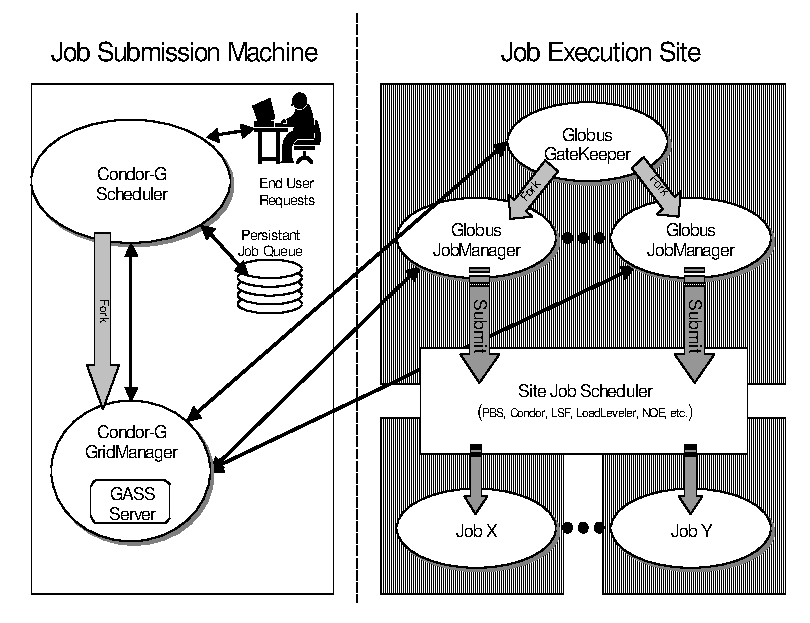
\psfig{width=\textwidth,file=condor-g/gfig1.eps}}
%\centerline{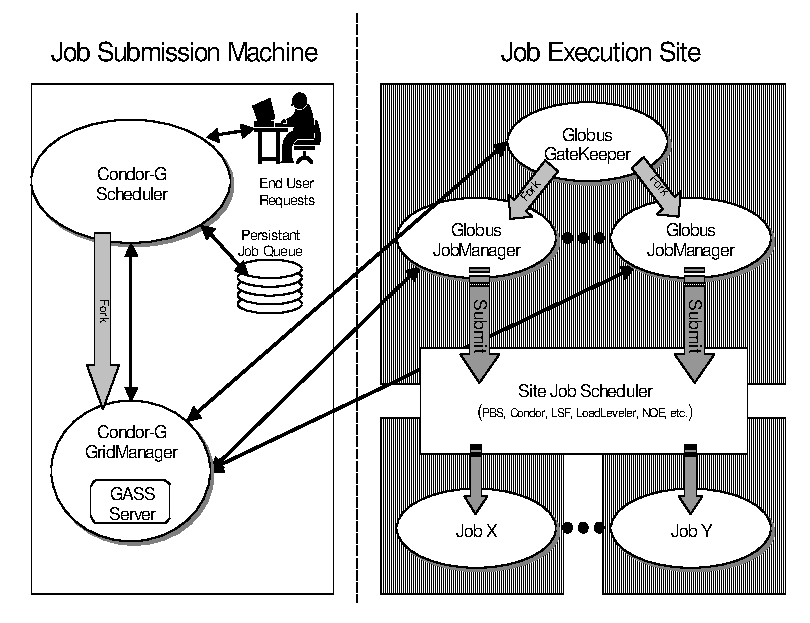
\includegraphics[clip]{condor-g/gfig1.eps}}
\centerline{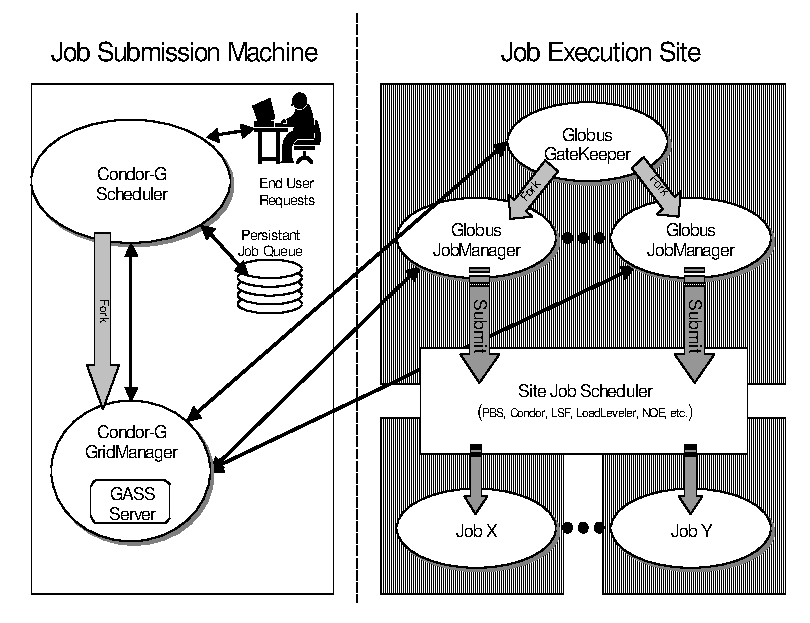
\includegraphics{condor-g/gfig1.eps}}
\caption{\label{fig:condorg}Remote Execution by Condor-G on Globus managed resources}
\end{figure}

Figure ~\ref{fig:condorg} shows how Condor-G interacts with Globus protocols.
Condor-G contains a GASS server, used to transfer the executable,
\File{stdin}, \File{stdout}, and \File{stderr} to and from
the remote job execution site.
Condor-G uses the GRAM protocol to contact the remote Globus Gatekeeper
and request that a new job manager be started.
GRAM is also used to monitor the job's progress.
Condor-G detects and intelligently handles cases
such as if the remote Globus resource crashes.

\subsection{Running a Globus Job}
\index{job!submission}

Under Condor, successful job submission to the Globus universe requires
credentials.
An X509 certificate is used to create a proxy,
and an account, authorization, or allocation to use a grid resource
is required.
For more information on proxies and certificates,
please consult the Alliance PKI pages at 

\Url{http://archive.ncsa.uiuc.edu/SCD/Alliance/GridSecurity/}

Before submitting a job to Condor under the Globus universe,
make sure you have your Grid 
credentials and have used \Prog{grid-proxy-init} to create a proxy.

A job is submitted for execution to Condor using the
\Condor{submit} command.
\index{Condor commands!condor\_submit}
\Condor{submit} takes as an argument the name of a file called a submit description file.
\index{submit description file!Globus universe}
The following sample submit description file will run a job on
the Origin2000 at NCSA.

\begin{verbatim}
executable = test
globusscheduler = modi4.ncsa.uiuc.edu/jobmanager
universe = globus
output = test.out
log = test.log
queue
\end{verbatim} 

The 
\AdAttr{executable}
for this example is
transferred from the local machine to the remote machine.
By default, Condor transfers the executable.
Note that this executable must be compiled for the correct
platform.

The \AdAttr{globusscheduler} command is dependent on the
scheduling software available on remote resource.
This command will change based on the Grid resource
intended for execution of the job.

No input file is specified for this example job.
Condor transfers the output file produced 
from the remote machine to the local machine during execution.
The log file is maintained on the local machine.

To submit this job to Condor-G for execution on the
remote machine, use
\begin{verbatim}
condor_submit test.submit
\end{verbatim}
Where \File{test.submit} is the name of the submit description file.

Example output from 
\Condor{q} for this submission looks like:
\begin{verbatim}
% condor_q


-- Submitter: wireless48.cs.wisc.edu : <128.105.48.148:33012> : wireless48.cs.wi

 ID      OWNER         SUBMITTED     RUN_TIME ST PRI SIZE CMD
   7.0   epaulson     3/26 14:08   0+00:00:00 I  0   0.0  test

1 jobs; 1 idle, 0 running, 0 held
\end{verbatim}

After a short time, Globus accepts the job.
Again running \Condor{q} will now result in

\begin{verbatim}
% condor_q


-- Submitter: wireless48.cs.wisc.edu : <128.105.48.148:33012> : wireless48.cs.wi

 ID      OWNER         SUBMITTED     RUN_TIME ST PRI SIZE CMD
   7.0   epaulson     3/26 14:08   0+00:01:15 R  0   0.0  test

1 jobs; 0 idle, 1 running, 0 held
\end{verbatim}

Then, very shortly after that, the queue will be empty again:

\begin{verbatim}
% condor_q


-- Submitter: wireless48.cs.wisc.edu : <128.105.48.148:33012> : wireless48.cs.wi

 ID      OWNER            SUBMITTED     RUN_TIME ST PRI SIZE CMD

0 jobs; 0 idle, 0 running, 0 held
\end{verbatim}


A second example of a submit description file runs the Unix \Prog{ls}
program on a different Globus resource.

\begin{verbatim}
executable = /bin/ls
Transfer_Executable = false
globusscheduler = vulture.cs.wisc.edu/jobmanager
universe = globus
output = ls-test.out
log = ls-test.log
queue
\end{verbatim} 

In this example, the executable (the binary) is pre-staged.
The executable is on the remote machine, and it is not to
be transferred before execution.
The command
\begin{verbatim}
Transfer_Executable = FALSE
\end{verbatim}
within the submit description file identifies the executable
as being pre-staged.
In this case, the 
\AdAttr{executable}
command gives the pathname to the executable on the remote machine.

%%%%%%%%%%%%%%%%%%%%%%%%%%%%%%%%%%%%%%%%%%%%%%%%%%%%%%%
\subsection{Configuration and Credential Management}
%%%%%%%%%%%%%%%%%%%%%%%%%%%%%%%%%%%%%%%%%%%%%%%%%%%%%%%

The following configuration file entries relate to submission of
jobs to Grid resources.

\begin{verbatim}
GRIDMANAGER             = $(SBIN)/condor_gridmanager
GRIDMANAGER_LOG         = $(LOG)/GridmanagerLog
MAX_GRIDMANAGER_LOG     = 64000
GRIDMANAGER_DEBUG       = D_SECONDS D_COMMAND
\end{verbatim} 

\AdAttr{GRIDMANAGER}
gives the pathname to the gridmanager daemon.
The 
\AdAttr{GRIDMANAGER\_LOG}
and
\AdAttr{MAX\_GRIDMANAGER\_LOG}
entries give the location of and how long
the log files may be.
\AdAttr{GRIDMANAGER\_DEBUG}
sets some debugging levels for the gridmananger daemon.


\begin{verbatim}
CRED_MIN_TIME_LEFT      = 8*60*60;
\end{verbatim} 
The interesting configuration setting for working with globus universe
jobs is
\AdAttr{CRED\_MIN\_TIME\_LEFT}.
Condor-G has this setting so that there is less chance that your
proxy will expire before your job completes.
Condor-G checks
\AdAttr{CRED\_MIN\_TIME\_LEFT}
to make sure that your proxy has at least this
much time remaining
before it will submit your job.
For example, if your job runs for a
half an hour and there is a 40 minute queue wait time,
you should make sure there are
at least 70 minutes of proxy lifetime remaining.
This configuration file entry is in seconds,
and defaults to 8 hours.
Currently only \Condor{submit} uses this entry.

\begin{verbatim}
GRIDMANAGER_CHECKPROXY_INTERVAL = 600
GRIDMANAGER_MINIMUM_PROXY_TIME = 180
\end{verbatim} 

These entries are for the gridmanager daemon, and they are relevant to
the newest job managers from the Globus 2.0 version of software.

Condor-G periodically checks for an updated proxy at
an interval of
\AdAttr{GRIDMANAGER\_CHECKPROXY\_INTERVAL}
seconds.
For example, if you create a 12-hour proxy, and then
6 hours later re-run \Prog{grid-proxy-init},
Condor-G will check the proxy within
this time interval, and use the new proxy it finds there.
The default interval is 10 minutes.

Condor-G also knows when the proxy of each job will expire,
and if the proxy is not refreshed before
\AdAttr{GRIDMANAGER\_MINIMUM\_PROXY\_TIME}
seconds before the proxy expires,
Condor-G will shut down.
In other words, if
\AdAttr{GRIDMANAGER\_MINIMUM\_PROXY\_TIME}
is 180, and the proxy is 3 minutes away from
expiring, Condor-G will attempt to safely shut down,
instead of simply losing
contact with the remote job because it is unable to authenticate it.
The default setting is 3 minutes (180 seconds).

